\documentclass[10pt,a4paper]{article}
\usepackage[utf8]{inputenc}
\usepackage{ae}
\usepackage[brazil]{babel}
\usepackage[vmargin=2cm,hmargin=2cm,columnsep=0.75cm]{geometry}
\usepackage{float,nonfloat}
\usepackage{graphicx,color}
\usepackage{subcaption}
\usepackage{amsmath}

\makeatletter
\let\@institution\empty
\def\institution#1{\def\@institution{#1}}
\renewcommand{\maketitle}{
    \begin{center}
        {\Large\bfseries\@title\par\medskip}
        {\large
            \begin{tabular}[t]{c}%
                \@author
        \end{tabular}\par\medskip}
        {\itshape\@institution\par}
        {\itshape\@date\par}
\end{center}}
\makeatother

\newcommand{\pixel}{\textit{pixel} }
\newcommand{\pixels}{\textit{pixels} }

\begin{document}
% ============================================================================

\title{MC920: Introdução ao Processamento de Imagem Digital\\Tarefa 4}
\author{
    \begin{minipage}{6cm}
        \centering
        Martin Ichilevici de Oliveira\\
        RA 118077
    \end{minipage}
    \and
    \begin{minipage}{6cm}
        \centering
        Rafael Almeida Erthal Hermano\\
        RA 121286
    \end{minipage}
}
\institution{Instituto de Computação, Universidade Estadual de Campinas}
\date{\today}

\maketitle

% ============================================================================

\section{Convolução}
Convolução é uma operação de vizinhança linear, ou seja, ela é uma função que transforma um pixel de acordo com o somatório ponderado dos vizinhos.
Portanto, pode ser expresso matematicamente:

\begin{equation}
    g(x,y) = \sum_{s = -a}^{a}\sum_{t = -b}^{b}w(s,t) f(x - s, y - t)
    \label{eq:conv_eq}
\end{equation}

Em que $a = \frac{m-1}{2}$ e $b = \frac{n-1}{2}$, onde $m$ e $n$ são o tamanho da janela da vizinhança, e $w(s,t)$ é uma função que determina o peso do vizinho.

\subsection{Propriedades}
A convolução é uma operação linear já que ela respeita a aditividade e a homogeneidade

\subsubsection{Aditividade}
\begin{center}
    $\begin{aligned}
        g(f+h) = &\sum_{s = -a}^{a}\sum_{t = -b}^{b}w(s,t) (f(x - s, y - t) + h(x - s, y - t)) \\
        g(f+h) = &\sum_{s = -a}^{a}\sum_{t = -b}^{b}w(s,t) f(x - s, y - t) + w(s,t) h(x - s, y - t)\\
        g(f+h) = &\sum_{s = -a}^{a}\sum_{t = -b}^{b}w(s,t) f(x - s, y - t) + \sum_{s = -a}^{a}\sum_{t = -b}^{b}w(s,t) h(x - s, y - t) \\
        g(f+h) = &g(f) + g(h)
    \end{aligned}$
\end{center}

\subsubsection{Homogeneidade}
\begin{center}
    $\begin{aligned}
        g(a f) = &\sum_{s = -a}^{a}\sum_{t = -b}^{b}w(s,t) a f(x - s, y - t) \\
        g(a f) = &a \sum_{s = -a}^{a}\sum_{t = -b}^{b}w(s,t) f(x - s, y - t) \\
        g(a f) = &a g(f)
    \end{aligned}$
\end{center}

\subsection{Aplicações}
\subsubsection{Blur}
O blur é utilizado para eliminar ruidos, removendo pequenos detalhes da imagem. O blur consiste em substituir cada pixel da imagem pela média dos vizinhos eliminando transições bruscas. Um possível problema na utilização do blur é a perda de definição nas bordas dificultando a identificação dos contornos.

\subsubsection*{Standard Average Blur}
Consiste em aplicar para todos os vizinhos o mesmo peso. Da equação \ref{eq:conv_eq} temos que $w(s,t) = \frac{1}{n \cdot m} \forall s,t$. Para uma vizinhança 3x3 temos que a máscara é:

\[ w(s,t) = \frac{1}{9} \cdot \left|
    \begin{array}{ccc}
        1 & 1 & 1 \\
        1 & 1 & 1 \\
        1 & 1 & 1 \\
\end{array}\right|\]

\subsubsection*{Weighted Average Blur}
Consiste em aplicar para os vizinhos 4 conexos um peso maior aos vizinhos 8 conexos. Portanto, para uma vizinhança 3x3 temos que a mascara é:

\[ w(s,t) = \frac{1}{16} \cdot \left|
    \begin{array}{ccc}
        1 & 2 & 1 \\
        2 & 4 & 2 \\
        1 & 2 & 1 \\
\end{array}\right|\]

\subsection{Implementação}
Foram usadas duas máscaras, $m_1$ e $m_2$:

\[
    m_1 = \frac{1}{5} \cdot \left|
    \begin{array}{ccc}
        0 & 1 & 0 \\
        1 & 1 & 1 \\
        0 & 1 & 0 \\
    \end{array}\right|
    \qquad
    m_2 = \frac{1}{4} \cdot \left|
    \begin{array}{ccc}
        0 & 1 & 0 \\
        0 & 1 & 1 \\
        0 & 1 & 0 \\
    \end{array}\right|
\]

Testou-se inicialmente na matriz $M$ abaixo:

\[
    M = \cdot \left|
    \begin{array}{ccccc}
                &    & \vdots \\
                & 10 & 10 & 10 \\
        \cdots  & 10 & 90 & 10 & \cdots\\
                & 10 & 10 & 10 \\
                &    & \vdots \\
    \end{array}\right|
\]
o que produziu (recortando as bordas):
\[
    M_1 = \frac{1}{5} \cdot \left|
    \begin{array}{ccc}
        10 & 26 & 10 \\
        26 & 26 & 26 \\
        10 & 26 & 10 \\
    \end{array}\right|
    \qquad
    M_2 = \frac{1}{4} \cdot \left|
    \begin{array}{ccc}
        10 & 30 & 10 \\
        10 & 30 & 30 \\
        10 & 30 & 10 \\
    \end{array}\right|
\]

Aplicou-se então a convolução com as matrizes acima referidas à Figura \ref{fig:original}. Os resultados estão nas Figuras \ref{fig:dst1} e \ref{fig:dst2}.
\begin{figure}[!ht]
    \centering
    \begin{subfigure}[ht]{0.45\textwidth}
        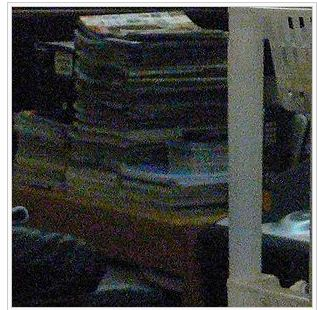
\includegraphics[width=\textwidth]{original.jpg}
        \caption{Figura original\cite{image}}
        \label{fig:original}
    \end{subfigure}
    \qquad
    \begin{subfigure}[ht]{0.45\textwidth}
        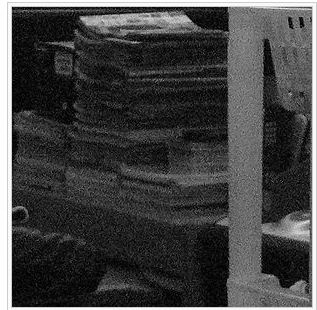
\includegraphics[width=\textwidth]{src.jpg}
        \caption{Convertida para tons de cinza}
        \label{fig:src}
    \end{subfigure}
    \\
    \begin{subfigure}[ht]{0.45\textwidth}
        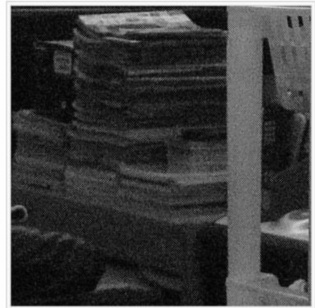
\includegraphics[width=\textwidth]{dst1.jpg}
        \caption{Após convolução 1}
        \label{fig:dst1}
    \end{subfigure}
    \qquad
    \begin{subfigure}[ht]{0.45\textwidth}
        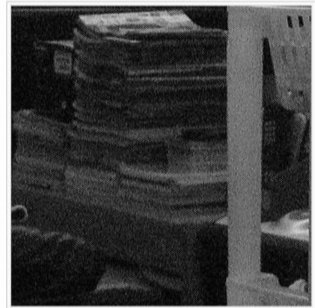
\includegraphics[width=\textwidth]{dst2.jpg}
        \caption{Após convolução 2}
        \label{fig:dst2}
    \end{subfigure}
    \caption{Imagem original e em tons de cinza antes e após convolução}
\end{figure}
\section{Limiarização}
Consiste em escurecer os pixels que possuem nível de cinza abaixo de M e clarear imagens com nível de cinza acima de M. O resultado final desta operação é uma imagem binária. Aplicou-se o procedimento à Figura \ref{fig:original2} (convertida para tons de cinza na Figura \ref{fig:src_thr}), e o resultado pode ser observado em \ref{fig:dst_thr}.
\begin{align*}
    T[f(x,y)] &= 0 \text{ se } f(x,y) < M \\
              &= 1 \text{ se } f(x,y) > M
\end{align*}

\begin{figure}[!ht]
    \centering
    \begin{subfigure}[ht]{0.45\textwidth}
        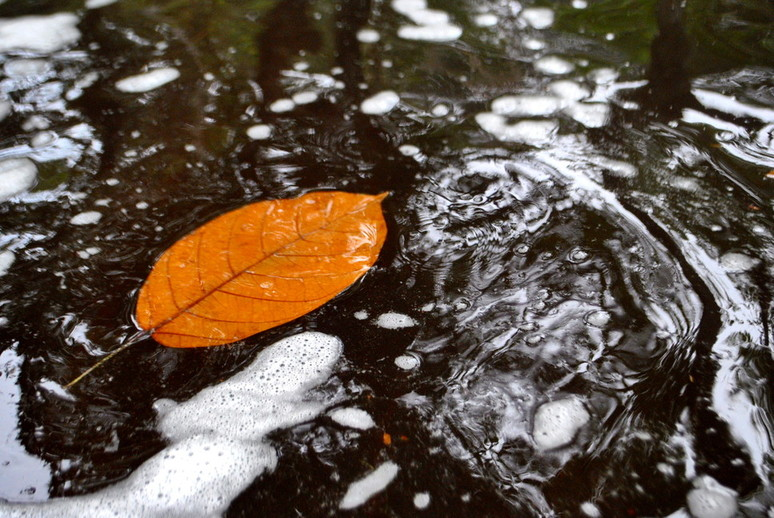
\includegraphics[width=\textwidth]{original2.jpg}
        \caption{Figura original}
        \label{fig:original2}
    \end{subfigure}
    \\
    \begin{subfigure}[ht]{0.45\textwidth}
        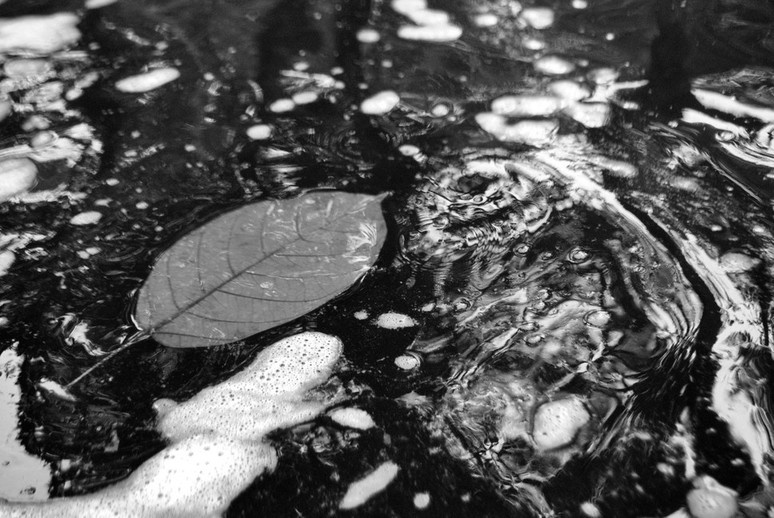
\includegraphics[width=\textwidth]{src_thr.jpg}
        \caption{Convertida para tons de cinza}
        \label{fig:src_thr}
    \end{subfigure}
    \qquad
    \begin{subfigure}[ht]{0.45\textwidth}
        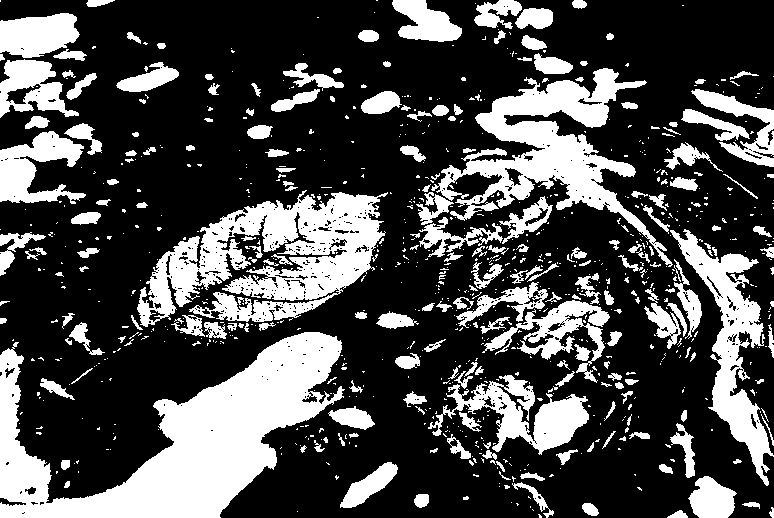
\includegraphics[width=\textwidth]{dst_thr.jpg}
        \caption{Após limiarização}
        \label{fig:dst_thr}
    \end{subfigure}
    \caption{Imagem original e em tons de cinza antes e após limiarização}
\end{figure}

\begin{thebibliography}{99}
    \bibitem{livro} GONZALEZ, Rafael C.; WOODS, Richard E.. \textbf{Digital Image Processing}. 3. ed. Upper Saddle River, NJ, EUA: Prentice-hall, 2006.
    \bibitem{image} \texttt{http://robotix.in/tutorials/category/opencv/noise\_reduction}
\end{thebibliography}

\end{document}
